\documentclass[twoside]{fksserie}
    
\setcounter{year}{25}
\setcounter{batch}{2}
\deadline{20.~září~2011 18.00}



\begin{document}


\maketitle

%\input{uvod\thebatch.tex}

\problemsheading % section

%\problemtask
%\problemtask

\solutionheading %section

Tady je ano\,ne vs. ano ne. Rovnice na více řádku
$
\sqrt{\frac{a+b+c}{\eu}} + \sqrt{\frac{a+b+c}{\eu}} =
\sqrt{\frac{a+b+c}{\eu}} + 1 =
1 + \sqrt{\frac{a+b+c}{\eu}} =
\pi + \sqrt{\frac{a+b+c}{\eu}} =
\sqrt{\frac{a+b+c}{\eu}} + \sqrt{\frac{a+b+c}{\eu}} =
\sqrt{\frac{a+b+c}{\eu}} + \eu =
\sqrt{\frac{a+b+c}{\eu}} + \sqrt{\frac{a+b+c}{\eu}} =
\sqrt{\frac{a+b+c}{\eu}} = \sqrt{\frac{a+b+c}{\eu}}
$

Tady následuje víceřádkové odvození
\eq[m]{
 f(x) = (x+a)(x+b) \lbl{eq:rce1}\\
 = x^2 + (a+b)x + ab\,.
}

Tady následuje víceřádkové odvození
\[
 f(x) = (x+a)(x+b)\,. \label{eq:rce2}
\]

Tady následuje víceřádkové odvození
\eq{
 f(x) = (x+a)(x+b)\,. \lbl{eq:rce3}
}

Rychlost se měří v \jd{m/s} také se dá napsat \popi{v}{m.s^{-1}} a čas v $\jd{s}$.



%\problemsolution
%\problemsolution


Vzpomeneme si na Keplerův třetí zákon, který dává do vztahu oběžné 
doby planet $T$ obíhající centrální slunce s~jejich hlavními 
poloosami $a$. V rovnici \eqref{eq:rce1} bude platit i v~našem případě pro změnu
trajektorie Země
\eq{
	\frac{T_0^2}{a_0^3} = \frac{T_1^2}{a_1^3} \, \ztoho \, a_1 =
	\root 3 \of{ \frac{T_1^2}{T_0^2} } \, a_0 \, ,
}
kde indexy 0 budeme značit počáteční situaci, kdy Země obíhá Slunce
po kružnici s~polo\-měrem~$a_0 = "1 AU" = "1,50e11 m"$ s~oběžnou dobou~$T_0 =
"365,2 dne"$,
a indexy 1 budou značené veličiny odpovídající 
situaci po změně zemské dráhy (doba oběhu~$T_1 = "372,2 dne"$).
% \begin{wrapfigure}{r}{0.35\textwidth}
%   \begin{center}
%     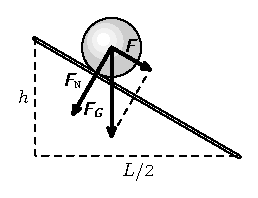
\includegraphics[width=0.33\textwidth]{obrazek.eps}
%   \end{center}
%   %\caption{Nakloněná rovina}
% \end{wrapfigure}
\illfig{obrazek.eps}{}{}

Vzhledem k~tomu, že přechod na eliptickou%
\footnote{Případně více eliptickou, pokud bychom se rovnou
rozhodli uvažovat i to, že původní dráha Země je ve skutečnosti
eliptická s~excentricitou~$e = 0,0167$.}
dráhu se uskutečnil rychle a ve směru pohybu Země, což znamená, že
přísluní (perihelium) nové dráhy bude ve vzdálenosti $a\_p = a_0$ od 
Slunce a~odsluní (afelium) bude ve vzdálenosti~$ a\_a = 2 a_1 - a_0 = \( 2 \root 3\of{ {T_1^2}/{T_0^2} } - 1 \) a_0 \approx  "1,025 AU"$.
Už z~tohoto výsledku je vidět, že dramatické změny teplot
v~průběhu roku nebudou nastávat, protože excentricita této dráhy je
pouze~$e_1 = {(a\_a - a\_p)}/{(a\_a + a\_p)} = 1 - 
\root 3\of{{T_0^2}/{T_1^2}} = 0,0126$, což je menší excentricita, 
než má Země ve~skutečnosti. Pokud bychom ale uvažovali eliptickou 
dráhu, záleželo by na tom, kdy v~průběhu roku dojde ke změně 
dráhy. Excentricita by se pak mohla i zmenšit, střední vzdálenost
Země-Slunce by vzrostla v~každém případě tak, aby se velká poloosa
zvětšila z~$a_0$ na~$a_1$.

Hustota toku sluneční energie ve vzdálenosti~$"1 AU"$ od Slunce se
nazývá {\it sluneční konstanta} a její hodnota je~$S_0 = "1370 W/m^2"$. Ve 
skutečnosti se nejedná o~konstantu, protože v~průběhu roku kolísá
o~cca~$"1,7 \%"$%
\footnote{Nemluvě o~tom, že se i její střední hodnota 
periodicky mění v~průběhu 11letého slunečního cyklu.},
ale v~rámci řešení úlohy
ji budeme považovat za konstantní. Hustota toku sluneční energie je 
nepřímo úměrná druhé mocnině vzdálenosti a~ve vzdálenosti~$r$ od 
Slunce ji můžeme vypočítat podle vztahu
\eq{
S_r = \frac{a_0^2}{r^2} S_0 \, .
}
V~přísluní naší nové dráhy je $S\_p = S_0$ z~definice a~v~odsluní
\eq{
S\_a = \frac{a\_p^2}{a\_a^2} S_0 = \frac{1}{\( 2 
\root 3\of{ {T_1^2}/{T_0^2} }-1\)^2} S_0 = "0.95" S_0 = 
"1300 W.m^{-2}" \, .
}

Pro odhad teploty budeme předpokládat, že Země je dokonale černé 
těleso a že v~každý okamžik je vyrovnaná bilance zářivého výkonu 
dopadajícího na Zemi a výkonem, která je Zemí vyzařovaná jako 
černým tělesem. Jedná se o~logický předpoklad, protože jinak by Země
nebyla v~tepelné rovnováze a~buď by se neustále ohřívala, nebo 
ochlazovala. Ve skutečnosti má Země tepelnou kapacitu, takže není 
v~tak dokonalé tepelné rovnováze -- ani blízko takové, že by se 
dopadající záření z~jedné strany na Zem okamžitě vyzařovalo všemi 
směry, ale berme to jako první přiblížení. Světelný výkon dopadající
na Zemi, která je dokonalá koule o~poloměru~$R\_Z$, ve vzdálenosti~$r$,
je úměrný průřezu Země a hustotě toku sluneční energie, $
P_r = \pi R\_Z^2 S_r \,.  
$
Výkon, který Země vyzáří na svém celém povrchu (obrázek \ref{fig:rel}), je dle 
Stefanova-Boltzmannova zákona 
\eq{
P = 4 \pi R\_Z^2 M = 4 \pi R\_Z^2 \sigma \tau^4 \, ,
}
kde~$M$ je intenzita vyzařování z~povrchu černého tělesa, $\sigma
= "5,67e-8 W.m^{-2}.K^{-4}"$ Stefanova-Boltzmannova konstanta 
a~$\tau$ je teplota černého tělesa. Vzhledem k~tomu, že se mají 
oba výkony rovnat, dostáváme vzorec pro teplotu Země v~našem přiblížení
\eq{
\tau_r = \root 4\of{\frac{S_r}{4 \sigma}} = \sqrt{\frac{a_0}{2 r}} 
\root 4\of{\frac{S_0}{\sigma}} \,.
}
Teplota v~perihelu pak vyjde $\tau\_p \approx "6 \C"$ a v~afelu $\tau\_a \approx
"2 \C"$. Teplota v~perihelu by teoreticky podle našich předpokladů
měla odpovídat střední teplotě na Zemi v~průběhu roku, která se udává
jako~$"14 \C"$. Což na první pohled úplně nesedí, ale vzhledem k~počtu
zanedbání, kterých jsme se dopustili, je to poměrně dobrá shoda. Další 
vlivy, které by se pro správné určení teploty měly započítat, jsou 
například to, že ve skutečnosti spektrum Země při vyzařování nebude 
ideálně odpovídat vyzařování černého tělesu, ale mělo by určitou 
specifickou vyzařovací charakteristiku, navíc i tato celková 
charakteristika by byla jenom přiblížením, protože Země není jenom 
z~jedné chemické látky, ale jinak bude vyzařovat pevnina a jinak 
oceány. Toto by vedlo spíš ke snížení očekávané teploty Země. Vliv na
teplotu Země má také to, že má horké jádro -- částečně obsahující 
tepelnou energii od doby vzniku Země pocházející z~gravitační
potenciální energie a dále v~jádru dochází k~rozpadu radioaktivních 
prvků, což také zvyšuje teplotu Země.
Další věcí je přítomnost atmosféry, která díky skleníkovým
plynům zvyšuje teplotu zemského povrchu.

\fullfig{obrazek.jpg}{Reliktní záření}{fig:rel}

\section{Něco navíc}

Pokud bychom tedy chtěli vyřešit globální oteplování jako ve Futuramě,
kde roboti ovlivnili dráhu Země tak, že rok byl o~týden (robotí pařby)
delší, tak by nás kromě výkyvů teploty v~průběhu roku zejména zajímala
průměrná roční teplota. Respektive i~s~naším relativně primitivním modelem
bychom mohli určit, o~kolik zhruba stupňů by se teplota změnila vůči 
původní teplotě. Za tím účelem můžeme využít druhý Keplerův zákon -- {\it zákon
ploch} -- říkající, že za jednotku času průvodič planety opíše stejnou plochu.%
\footnote{Je to jen jiná formulace zákona zachování momentu hybnosti.}
Pro plošnou rychlost~$w$ pak platí
\eq{
w = \frac{a_1 b_1}{T_1} = \frac{r v_r}{2} ,
}
kde~$b_1$ je vedlejší poloosa elipsy a~$v_r$ je rychlost planety ve 
vzdálenosti~$r$ od Slunce. Pokud bychom chtěli, můžeme vypočítat
i~hodnotu~$w$ s~pomocí vztahu $e = {\sqrt{a_1^2 - b_1^2}}/{a_1}$, 
která pak bude $w = \sqrt{a\_a a\_p} = a_0 
\sqrt{2 \left( {T_1}/{T_0} \right) ^{2/3} -1 }$, ale toto číslo
nebudeme dál potřebovat. Vystačíme~si s~úvahou, že když $w$ je 
konstantní, můžeme vyjádřit oběžnou rychlost jako funkci vzdálenosti~$v_r =
{2w}/{r}$.
Vzhledem k~tomu, že trajektorie Země je elipsa,
můžeme si vybrat souřadnou soustavu, kde Slunce bude v~jejím počátku
a~perihelium bude na ose~$x$ v~kladném směru. Naši elipsu popíšeme v~polárních 
souřadnicích jako 
\eq{
r_\phi = a_1 - (a_1 - a_0) \cos \phi \, ,
}
kde~$\phi$ je úhel měřený právě od perihelu v~kladném smyslu (proti směru 
hodinových ručiček). Jde o aproximaci pro malé excentricity $\epsilon$. 
Obecně můžeme kuželosečky v polárních souřadnicích zapsat ve tvaru 
\eq{
r(\phi) = \frac{a_0}{1-\epsilon\cos\phi}\,,
}
kde $a_0$ je velikost hlavní poloosy a $\epsilon$ je excentricita. Pro 
$\epsilon=0$ jde o kružnici, pro $0<\epsilon<1$ jde o elipsu, pro 
$\epsilon=1$ jde o parabolu a pro $\epsilon>1$ to je jedna větev hyperboly.

Pokud jste se ještě s~polárními souřadnicemi nesetkali,
tak místo souřadnice~$x$ a~$y$ máme souřadnice~$r = \sqrt{x^2 + y^2}$ 
určující vzdálenost od počátku a~$\phi$, což je právě zmíněný úhel, pro
který platí $\phi = \tg {y}/{x}$.

Poslední úvaha se týká toho, že  teplotu bychom chtěli \uv{vystředovat} tak, že
bychom si rozdělili dráhu 
Země v~průběhu roku na malé kousíčky, kdy má skoro stejnou teplotu
určenou naším modelem, a~teplotu vynásobili časem, za který Země příslušný
kousíček dráhy urazila. Všechny tyto vynásobené kousky bychom pak sečetli
a~vydělili dobou oběhu. Vlastně bychom spočítali vážený průměr teploty. 
Čas, který Zemi potrvá, než urazí nějakou dráhu, je 
nepřímo úměrný její rychlosti. Rychlost je zase v~našem případě nepřímo
úměrná vzdálenosti od Slunce, takže čas je úměrný vzdálenosti. Takže
můžeme jako váhovou funkci použít vzdálenost a ne přímo čas. Také
bude lepší, když kousíčky, ve kterých považujeme rychlost Země za konstantní,
půjdou k~nekonečně krátkým dobám -- tzn. přejdeme k~integrování. 
Průměrná teplota bude 
\eq{
\bar{\tau} =
\frac{\int_0^{2 \pi} r_\phi \tau_{r_\phi} \, \d\phi }{\int_0^{2 \pi} r_\phi \,
\d\phi } \, .
}
Tyto integrály si můžeme nechat numericky spočítat%
\footnote{Například pomocí stroje na~\url{http://www.wolframalpha.com/}.}
a~vyjde nám, že nemůžeme čekat změnu průměrné roční teploty ani o~celé~$"2 \C"$, 
takže pokud by bylo potřeba Zemi ochladit v~situaci, kdy by bylo všem 
nechutné vedro, ani o~týden delší rok by nestačil.


\seriesheading{Aplikace teorie konformních zobrazení} %section
\subsection{Od elektrostatiky k dynamice}
text seriálu.

\subsection{Od magentoelektrostatiky ke statice}
text další kapitoly seriálu.

\subsection{Od elektrostatiky k dynamice}
text seriálu.

\subsection{Od magentoelektrostatiky ke statice}
text další kapitoly seriálu.

\subsection{Od elektrostatiky k dynamice}
text seriálu.

\subsection{Od magentoelektrostatiky ke statice}
text další kapitoly seriálu.

\listoffigures


\makefooter % adreasa a patička

\end{document}
